%Version 3 October 2023
% See section 11 of the User Manual for version history
%
%%%%%%%%%%%%%%%%%%%%%%%%%%%%%%%%%%%%%%%%%%%%%%%%%%%%%%%%%%%%%%%%%%%%%%
%%                                                                 %%
%% Please do not use \input{...} to include other tex files.       %%
%% Submit your LaTeX manuscript as one .tex document.              %%
%%                                                                 %%
%% All additional figures and files should be attached             %%
%% separately and not embedded in the \TeX\ document itself.       %%
%%                                                                 %%
%%%%%%%%%%%%%%%%%%%%%%%%%%%%%%%%%%%%%%%%%%%%%%%%%%%%%%%%%%%%%%%%%%%%%

%%\documentclass[referee,sn-basic]{sn-jnl}% referee option is meant for double line spacing

%%=======================================================%%
%% to print line numbers in the margin use lineno option %%
%%=======================================================%%

% \documentclass[lineno,sn-basic]{sn-jnl}% Basic Springer Nature Reference Style/Chemistry Reference Style

%%======================================================%%
%% to compile with pdflatex/xelatex use pdflatex option %%
%%======================================================%%

\documentclass[pdflatex,sn-basic, Numbered]{sn-jnl}% Basic Springer Nature Reference Style/Chemistry Reference Style

%%Note: the following reference styles support Namedate and Numbered referencing. By default the style follows the most common style. To switch between the options you can add or remove �Numbered� in the optional parenthesis. 
%%The option is available for: sn-basic.bst, sn-vancouver.bst, sn-chicago.bst%  

% \documentclass[sn-nature]{sn-jnl}% Style for submissions to Nature Portfolio journals
% \documentclass[sn-basic]{sn-jnl}% Basic Springer Nature Reference Style/Chemistry Reference Style
% \documentclass[sn-mathphys-num]{sn-jnl}% Math and Physical Sciences Numbered Reference Style 
%%\documentclass[sn-mathphys-ay]{sn-jnl}% Math and Physical Sciences Author Year Reference Style
% \documentclass[sn-aps]{sn-jnl}% American Physical Society (APS) Reference Style
%\documentclass[sn-vancouver,Numbered]{sn-jnl}% Vancouver Reference Style
%%\documentclass[sn-apa]{sn-jnl}% APA Reference Style 
%%\documentclass[sn-chicago]{sn-jnl}% Chicago-based Humanities Reference Style

%%%% Standard Packages
%%<additional latex packages if required can be included here>

\usepackage{graphicx}%
\usepackage{multirow}%
\usepackage{amsmath,amssymb,amsfonts}%
\usepackage{amsthm}%
\usepackage{mathrsfs}%
\usepackage[title]{appendix}%
\usepackage{xcolor}%
\usepackage{textcomp}%
\usepackage{manyfoot}%
\usepackage{booktabs}%
\usepackage{algorithm}%
\usepackage{algorithmicx}%
\usepackage{algpseudocode}%
\usepackage{listings}%
\usepackage{multicol}

\usepackage{caption}
\usepackage{placeins}
\usepackage{lipsum}
\usepackage{float}
\usepackage{csquotes}
%%%%

\renewcommand{\floatpagefraction}{0.5}
\renewcommand{\textfraction}{0.1}
%%%%%=============================================================================%%%%
%%%%  Remarks: This template is provided to aid authors with the preparation
%%%%  of original research articles intended for submission to journals published 
%%%%  by Springer Nature. The guidance has been prepared in partnership with 
%%%%  production teams to conform to Springer Nature technical requirements. 
%%%%  Editorial and presentation requirements differ among journal portfolios and 
%%%%  research disciplines. You may find sections in this template are irrelevant 
%%%%  to your work and are empowered to omit any such section if allowed by the 
%%%%  journal you intend to submit to. The submission guidelines and policies 
%%%%  of the journal take precedence. A detailed User Manual is available in the 
%%%%  template package for technical guidance.
%%%%%=============================================================================%%%%

%% as per the requirement new theorem styles can be included as shown below
\theoremstyle{thmstyleone}%
\newtheorem{theorem}{Theorem}%  meant for continuous numbers
%%\newtheorem{theorem}{Theorem}[section]% meant for sectionwise numbers
%% optional argument [theorem] produces theorem numbering sequence instead of independent numbers for Proposition
\newtheorem{proposition}[theorem]{Proposition}% 
%%\newtheorem{proposition}{Proposition}% to get separate numbers for theorem and proposition etc.

\theoremstyle{thmstyletwo}%
\newtheorem{example}{Example}%
\newtheorem{remark}{Remark}%
\theoremstyle{thmstylethree}%
\newtheorem{definition}{Definition}%

\raggedbottom
%%\unnumbered% uncomment this for unnumbered level heads

\newcommand{\comment}[1]{\textcolor{purple}{#1}}

\begin{document}

\title[Article Title]{On the role of 24/7 carbon-free energy matching in accelerating advanced clean energy technologies}

%%=============================================================%%
%% GivenName	-> \fnm{Joergen W.}
%% Particle	-> \spfx{van der} -> surname prefix
%% FamilyName	-> \sur{Ploeg}
%% Suffix	-> \sfx{IV}
%% \author*[1,2]{\fnm{Joergen W.} \spfx{van der} \sur{Ploeg} 
%%  \sfx{IV}}\email{iauthor@gmail.com}
%%=============================================================%%

\author*[1]{\fnm{Iegor} \sur{Riepin}}\email{iegor.riepin@tu-berlin.de}
\author[1]{\fnm{Tom} \sur{Brown}}\email{t.brown@tu-berlin.de}
\author[2]{$<Princeton?>$}\email{$<Princeton?>$}
\author[3]{\fnm{Devon} \sur{Swezey}}\email{dswezey@google.com}

\affil[1]{\orgdiv{Department of Digital Transformation in Energy Systems}, \orgname{TU Berlin}, \orgaddress{Berlin, Germany}}

\affil[3]{\orgdiv{Global Energy and Climate}, \orgname{Google LLC}, \orgaddress{$<$city, country$>$}}

%%==================================%%
%% Sample for unstructured abstract %%
%%==================================%%

\abstract{

The early commitments to 24/7 carbon-free energy matching create an early market for advanced clean energy technologies like long-duration energy storage and clean firm generators. Companies and governments optimizing their energy procurement and investment strategies to match own consumption with clean electricity round-the-clock can play a catalytic role in innovation, financeability, and widespread availability of technologies required for a wider societal transition to secure, reliable and clean energy systems.
\\ 
\comment{Abstract two sentences for Nature Energy Comment paper.}
}

% \keywords{keyword1, Keyword2, Keyword3, Keyword4}

%%\pacs[JEL Classification]{D8, H51}

%%\pacs[MSC Classification]{35A01, 65L10, 65L12, 65L20, 65L70}

\maketitle

\comment{
A Comment is a flexible format, focusing on the scientific, commercial, ethical, legal, societal, or political issues surrounding research, or on other matters of policy, science and society related to energy. Comment articles should be topical, readable, provocative and introduce new concepts/points of view, providing a personal perspective on a matter of public or scientific importance. The main criteria are that they should be of immediate interest to a broad readership and should be written in an accessible, non-technical style. \href{https://www.nature.com/nenergy/content}{https://www.nature.com/nenergy/content}\\}
\comment{
\noindent Length -- up to 2,000 words; There are no specific structural guidelines; Commentaries do not normally contain primary research data; References should be used sparingly --- up to 15; Peer review is at the editors' discretion.\\
Length now: 1,000 words. \\ 
I must rely on lengthy captions to make main text less technical and wordy.
}


\subsection*{Big challenges ahead}\label{sec1}

Humanity faces a major challenge in mitigating the adverse impacts of climate change and related losses and damages to nature and people. A pathway to prevent the worst climate damages requires \textit{\enquote{a rapid and deep and, in most cases, immediate greenhouse gas emissions reductions in all sectors this decade}} \cite{ipccAR6SynthesisReport2023}. Global net human-caused emissions of carbon dioxide (CO$_2$) has to reach net zero by 2050 to keep us consistent with efforts to limit the long-term increase in average global temperatures to 1.5 °C.

The energy sector—a major culprit, responsible for approximately three-quarters of global greenhouse gas emissions—playing a pivotal role \cite{ieaNetZero20502021}. A growing political consensus and national climate initiatives are calling for a complete transformation of how we produce, transport, and consume energy. To achieve this goal, a significant expansion of all available  clean energy and technologies is necessary. According to the International Energy Agency (IEA), net-zero pathway requires a rapid scale-up of solar and wind power within this decade, aiming for annual additions of 630~GW of solar photovoltaics (PV) and 390~GW of wind by 2030, which would quadruple the record levels established in 2020 \cite{ieaNetZero20502021}.

It is a broad scientific consensus that reaching net zero by 2050 requires not only a massive scale-up of available clean technologies, but also a rapid research and development (R\&D) and large-scale deployment of advanced technologies that are not on the market yet \cite{sepulvedaRoleFirmLowCarbon2018, bistlineImpactCarbonDioxide2021, brownUltralongdurationEnergyStorage2023, ieaNetZero20502021}. Among them are clean firm generation technologies such as geothermal power, advanced nuclear generators, Allam-cycle gas generators with carbon capture and storage (CCS), as well as long-duration energy storage (LDES) technologies based on thermal, electrochemical, or mechanical principles. To bring these new technologies to market on a large scale in time, major efforts will be needed over the next decade.


\subsection*{The chasm of technology commercialization}\label{sec2}

Literature items
Google white paper: \citet{google-advancedtech}\\


Technology and financing risk

First of a Kind project development challenges

Securing long-term offtake agreements for FOAK projects can also be a challenge

Moving beyond FOAK projects

\subsection*{New trend: 24/7 CFE matching}\label{sec3}

what is 24/7 CFE matching

early movers

why it is important

early market

24/7 matching in selected country: Germany

\lipsum[1]

\FloatBarrier
\begin{figure}[htbp]
    \centering
    \includegraphics[width=0.85\textwidth]{images/dashboard_1.pdf}
    \captionsetup{width=0.85\textwidth}
    \caption{Illustrative modelling of 24/7 CFE matching.
    \textbf{Panel (a)} portfolio capacity procured by participating consumers,  
    \textbf{Panel (b)} cost breakdown of a procurement policy,
    \textbf{Panel (c)} Average emissions rate of participating consumers. 
    Here we assume Germany 2025 as an example location and participation rate of C\&I consumers in 24/7 CFE matching strategy at 5\% (ca. 1900~MW load). \\
    Notation: CFE scores 90\%, 98\% and 100\% correspond to the share of time when the electricity consumed by the participating consumers is carbon-free.
    P1: palette of technologies that are commercially available today: onshore wind, utility scale solar PV, and battery storage; P2: all above plus iron-air battery storage (100h duration); P3: all above plus an Allam cycle power plant with CCS.}\label{fig:dashboard}
\end{figure}
\FloatBarrier

\subsection*{Technology learning}\label{sec3}

Technology learning 

\FloatBarrier
\begin{figure}[htbp]
    \centering
    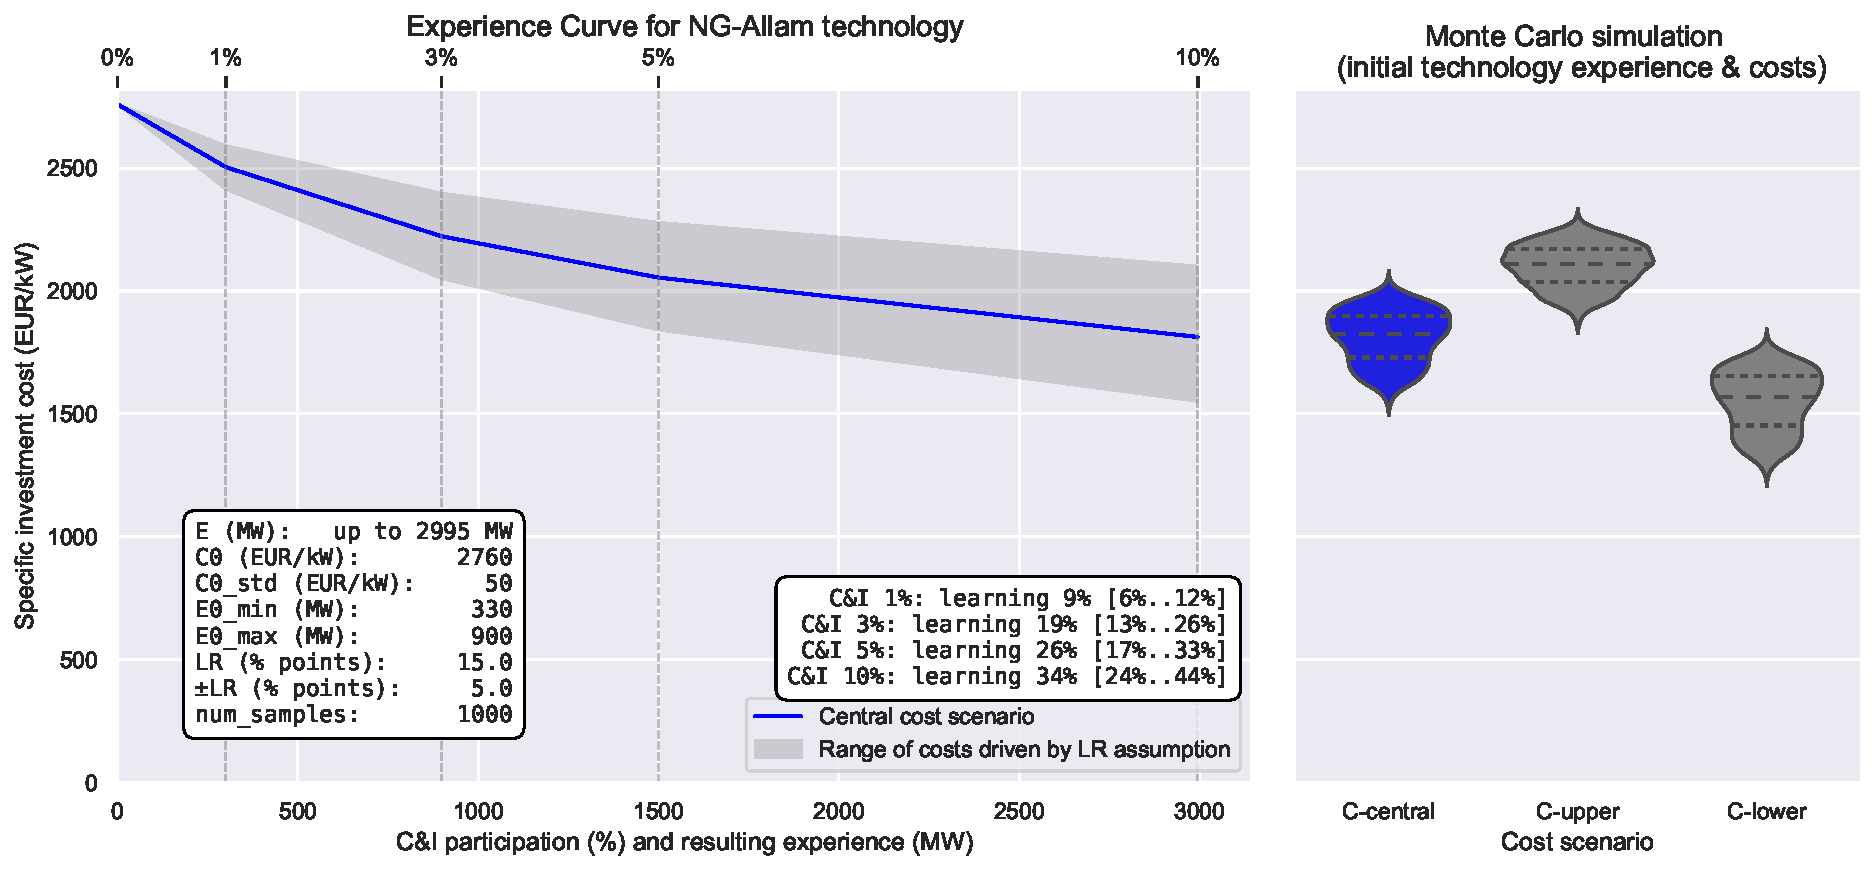
\includegraphics[width=\textwidth]{images/e_curve_NG-Allam.pdf}
    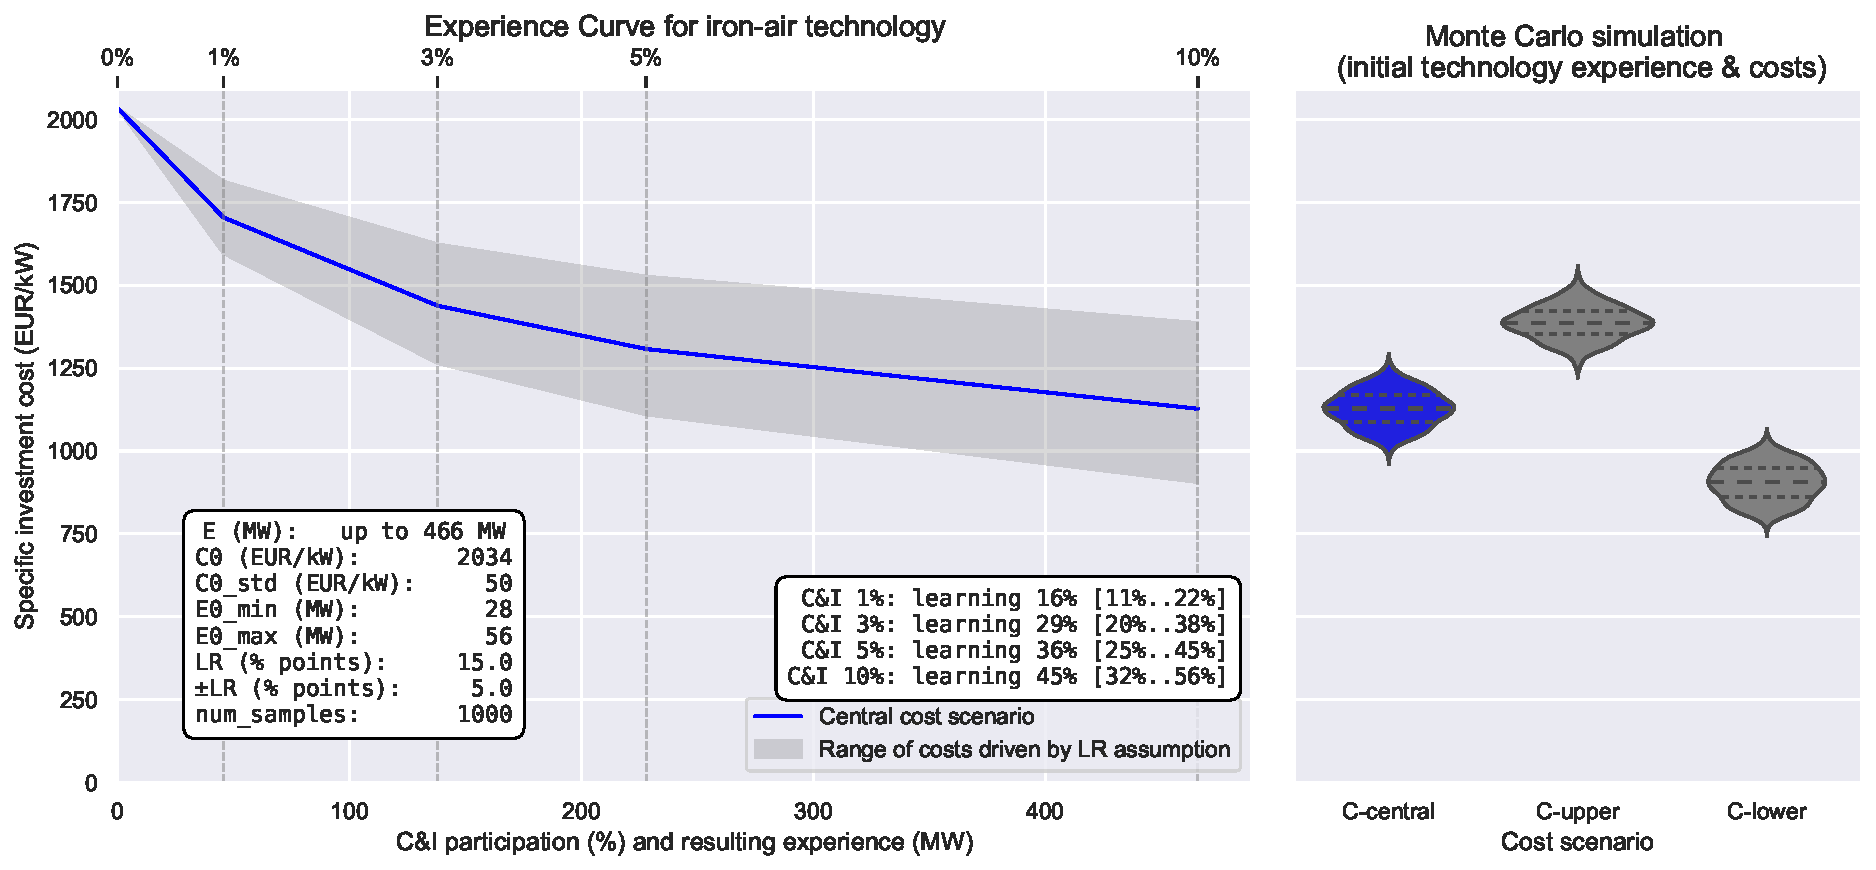
\includegraphics[width=\textwidth]{images/e_curve_iron-air.pdf}
    \caption{Technology learning curves for the NG-Allam power plant (\textbf{top panel}) and iron-air battery storage (\textbf{bottom panel}).
    The learning curves are based on the experience model with the technology investments based on 24/7 CFE model with varying C\&I participation level $[0\%..10\%]$ and learning rates of 15$\pm$5\%. \\
    For the Monte Carlo analysis calibration, the initial costs ($C0$) are sampled from a normal distribution with a mean based on our 2025 technology cost assumption and a standard deviation of 50~EUR/kW. Initial experience levels ($E0$) are sampled from a uniform distribution, with bounds derived from public information on projects planned to operate by 2025. In NG-Allam's model, initial experience lies between cases when one of three planned projects planned by 2025 is completed, and when all three projects are completed \cite{BroadwingEnergyProject, CoyoteCleanPower, FrogLakeProject}. In iron-air storage model, the distribution bounds are formed by assuming that 50\% to 100\% of the projects announced to operate by 2025 are realized on time \cite{FormEnergyLatest2024}.
    }
    \label{fig:panels}
\end{figure}
\FloatBarrier


\subsection*{System impact}\label{sec3}

Impact
\lipsum[1]

\FloatBarrier
\begin{figure}[htbp]
    \centering
    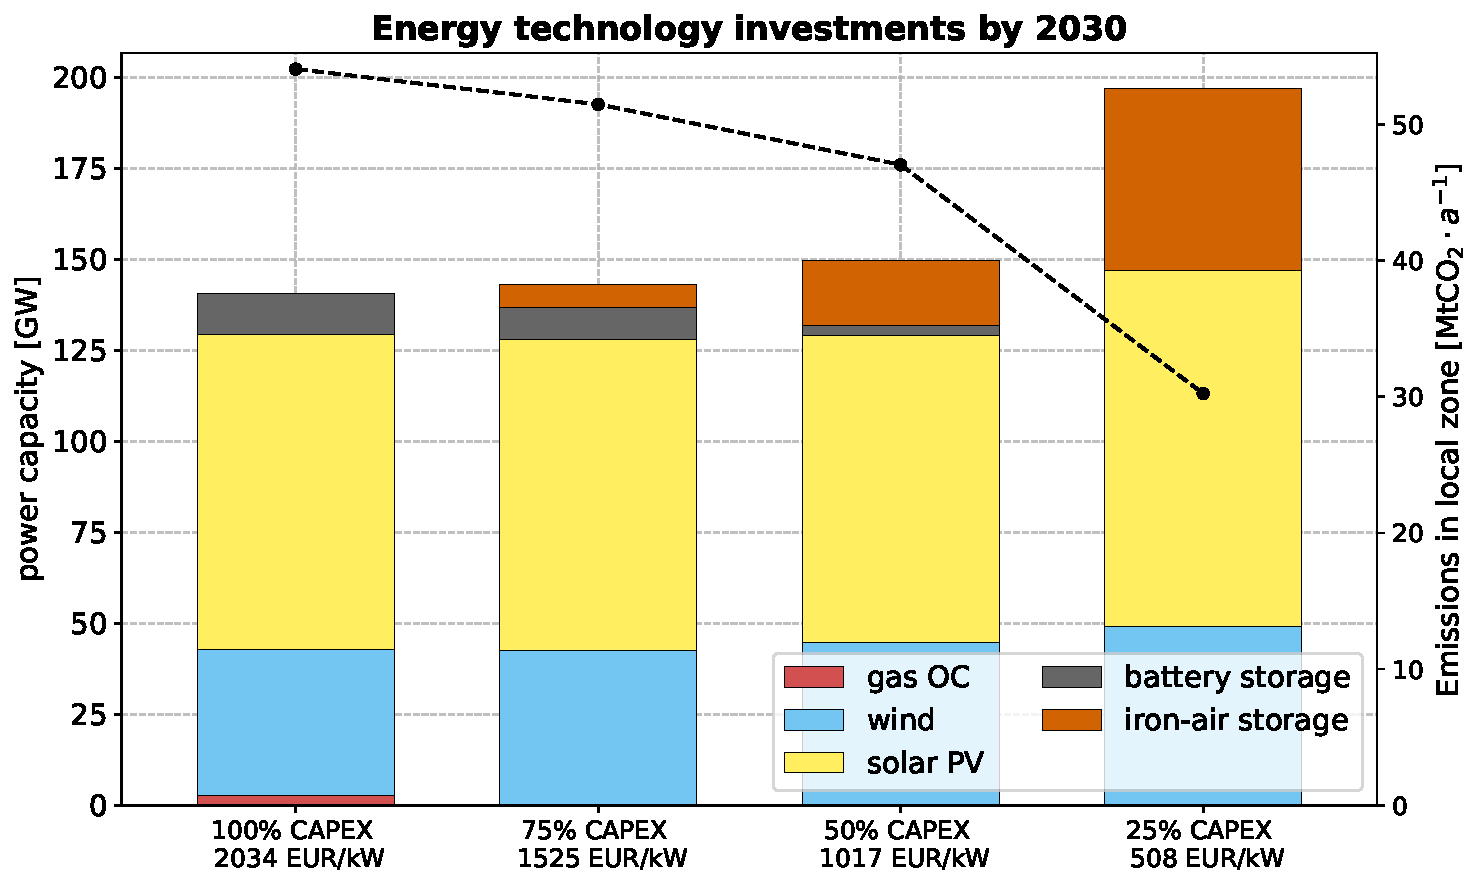
\includegraphics[width=0.7\textwidth]{images/dashboard_3.pdf}
    \captionsetup{width=0.7\textwidth}
    \caption{Power capacity investments and country emissions in German 2030 system as a function of CAPEX for iron-air battery storage. \\ 
    Here we assume no voluntary 24/7 CFE commitments, i.e., technology investments are driven by economic considerations only. Iron-air battery storage has a fixed duration of 100 hours \cite{FormEnergyLatest2024}. Price for EU ETS allowances is 100 EUR/tCO$_2$. Technology costs are based on \citet{DEA-technologydata} for 2030. Other background system assumptions are aligned with \citet{riepin-zenodo-systemlevel247}.}\label{fig:impact}
\end{figure}
\FloatBarrier


\subsection*{A broad perspective}\label{sec4} 

reducing costs of clean firm technologies benefits all:

- lower costs for 24/7 CFE matching for followers
- makes deep decarbonization more affordable and enables more ambitious climate goals
- energy security and resilience
- reduce curtailment, and the need for transmission and distribution infrastructure

%%%%%%%%%%%%%%%%%%%%%%%%%%%%%%%%%%%%%%%%%%%%%%%%%%%%%%%%
\backmatter

\bmhead{Acknowledgements} We thank the following people for insights and fruitful discussions: Elisabeth Zeyen, Adam Forni, Brian Denvir, and the participants of the 24/7 CFE Hub Meeting in May 2024. IR acknowledges a research grant from Google LLC.

\bmhead{Author contributions} The authors contributed equally to this work.

\bmhead{Code availability} The code to reproduce the illustrative experiments is available at GitHub under open licenses \cite{code247CFE}.

\bmhead{Competing interests} \comment{I suppose there is no competing interests to declare for this work from @TUB side, TB do you agree? @DS please suggest your line here.}


%%===========================================================================================%%
%% If you are submitting to one of the Nature Portfolio journals, using the eJP submission   %%
%% system, please include the references within the manuscript file itself. You may do this  %%
%% by copying the reference list from your .bbl file, paste it into the main manuscript .tex %%
%% file, and delete the associated \verb+\bibliography+ commands.                            %%
%%===========================================================================================%%

\bibliography{sn-bibliography}% common bib file
%% if required, the content of .bbl file can be included here once bbl is generated
%%\input sn-article.bbl

\end{document}
